\documentclass{article}
\usepackage{amsmath, tikz, enumerate, sfmath, bm, multicol, tcolorbox}
\renewcommand{\familydefault}{\sfdefault}
\usepackage[top = 0.5in, bottom = 0.5in, left = 1in, right = 1in]{geometry}
\pagestyle{empty}
\raggedright
\tikzset{>=stealth}
\begin{document}
\section*{Vectors and Matrices: Adding, Subtracting, and Scalar Multiplication}

\begin{tcolorbox}[colframe=orange!70!white, coltitle=black, title=\textbf{Summary}]
\begin{enumerate}
    \item A vector is a directed line segment.
    \item We can add or subtract vectors via corresponding elements if they have the same dimensions and we can multiply any vector by a scalar.
    \item Any vector can be written in terms of basis vectors $\hat{\imath}$ and $\hat{\jmath}$.
    \item Matrices are 2 or more vectors in the coordinate plane.
\end{enumerate}
\end{tcolorbox}
% \fbox{\textsc{Today I Can}: Perform arithmetic operations to vectors and matrices.}

\subsection*{Vectors}

Any point in the coordinate plane can be represented by a directed line segment called a \textbf{vector}. For instance, we can draw a vector from the origin to the point $(3,4)$ below: \newline\\
\begin{center}
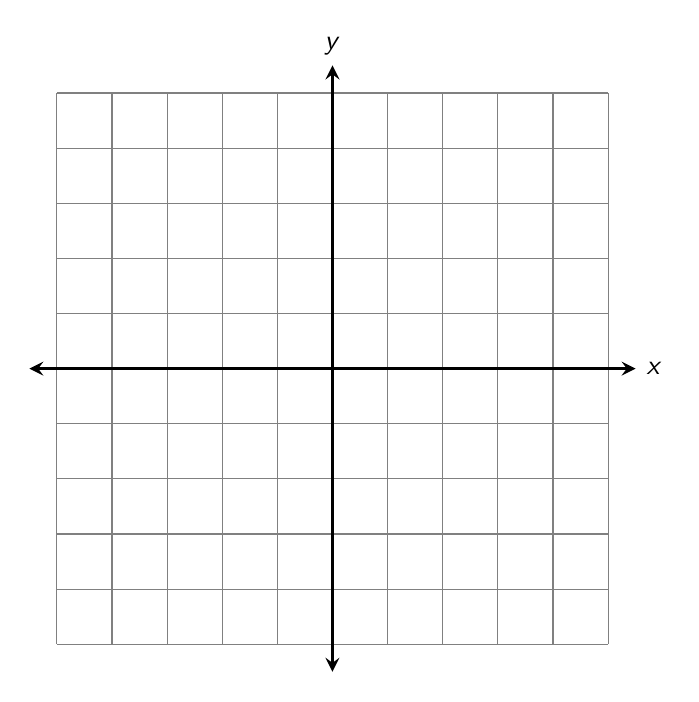
\begin{tikzpicture}[scale=0.7]
\draw[gray] (-5,-5) grid (5,5);
\draw[<->, very thick] (-5.5,0) -- (5.5,0) node [right] {$x$};
\draw[<->, very thick] (0,-5.5) -- (0,5.5) node [above] {$y$};
\end{tikzpicture}
\end{center}
\vspace{1in}

In the above picture, $\vec{v} = \begin{bmatrix}
3 \\ 4
\end{bmatrix}$, where $\vec{v}$ is a \textbf{column vector} with the dimensions 2 rows by 1 column.	\vspace{0.25in}

\emph{Note}: the values in the vector, 3 and 4, are called \textbf{elements}.

\newpage

\subsubsection*{Vector Addition}

We can add two vectors together if they have the same dimensions by adding their corresponding elements. \vspace{0.5in}

For instance, suppose $\vec{v} = \begin{bmatrix} 3 \\ 4\\ \end{bmatrix} \text{ and } \vec{w} = \begin{bmatrix} 2 \\ -3 \end{bmatrix}$	\quad then $\vec{v} + \vec{w}$ is   \vspace{2in}


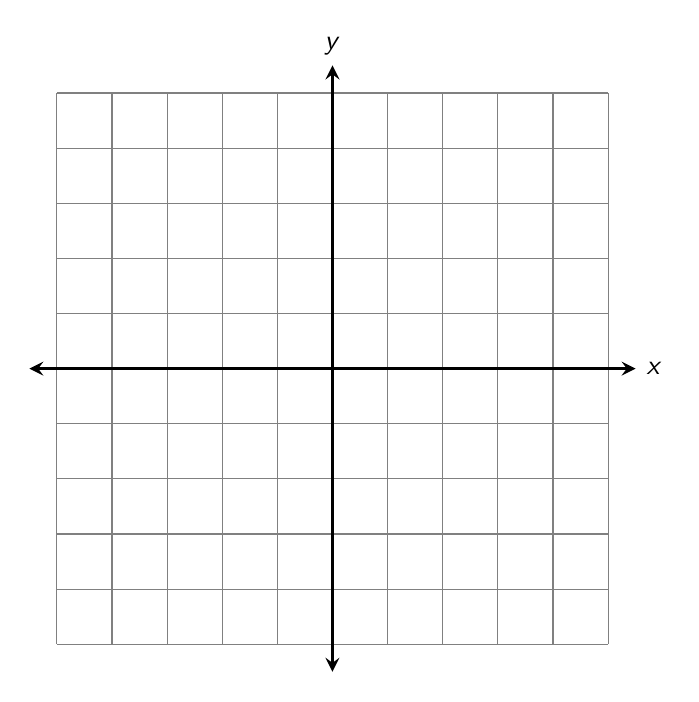
\begin{tikzpicture}[scale=0.7]
\draw[gray] (-5,-5) grid (5,5);
\draw[<->, very thick] (-5.5,0) -- (5.5,0) node [right] {$x$};
\draw[<->, very thick] (0,-5.5) -- (0,5.5) node [above] {$y$};
\end{tikzpicture}


\newpage

When we physically add vectors, we can move the second vector (without changing its shape or direction) so that it starts where the first ends:   \vspace{1in}

Visually, our previous problem of $\vec{v} = \begin{bmatrix}
3 \\ 4 \end{bmatrix} + \vec{w} = \begin{bmatrix} 2 \\ -3 \end{bmatrix}$ is \vspace{0.5in}

\begin{center}
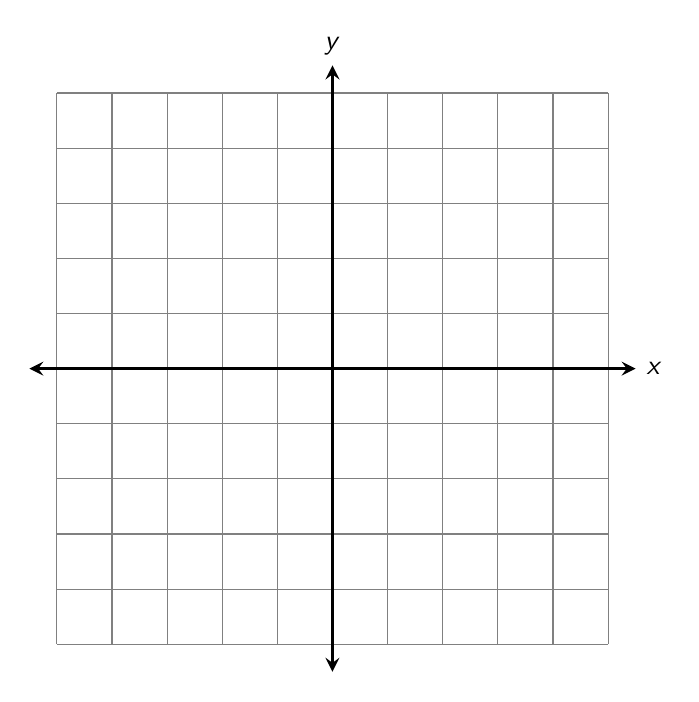
\begin{tikzpicture}[scale=0.7]
\draw[gray] (-5,-5) grid (5,5);
\draw[<->, very thick] (-5.5,0) -- (5.5,0) node [right] {$x$};
\draw[<->, very thick] (0,-5.5) -- (0,5.5) node [above] {$y$};
\end{tikzpicture}
\end{center}

\newpage

{\color{red}\textbf{Example 1.}} Find and graph the sum of the vectors below.

\[
\vec{v} = \begin{bmatrix}
-1 \\ 3
\end{bmatrix}
\quad \vec{w} = \begin{bmatrix}
-3 \\ 0
\end{bmatrix}
\]
\bigskip

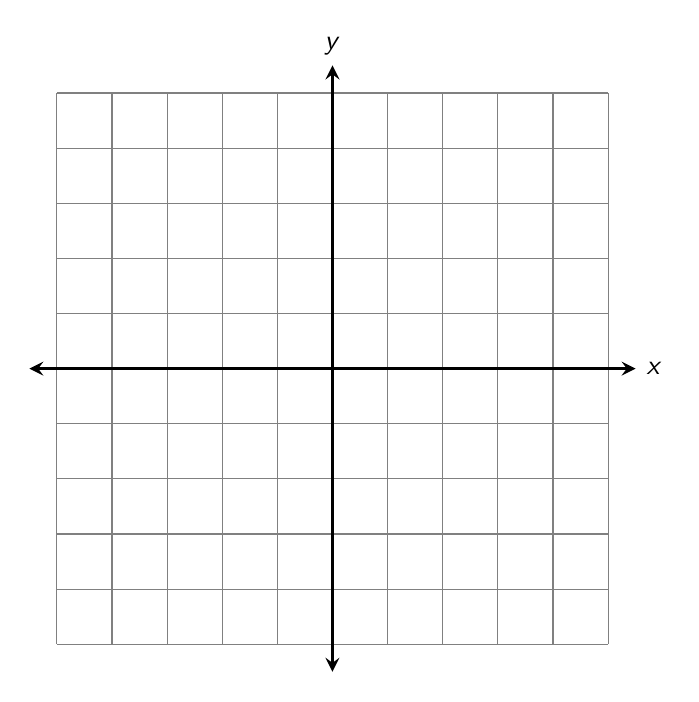
\begin{tikzpicture}[scale=0.7]
\draw[gray] (-5,-5) grid (5,5);
\draw[<->, very thick] (-5.5,0) -- (5.5,0) node [right] {$x$};
\draw[<->, very thick] (0,-5.5) -- (0,5.5) node [above] {$y$};
\end{tikzpicture}

\newpage



\subsubsection*{Scalar Multiplication}

A \textbf{scalar} is another name for a real number. \vspace{0.25in}

When we multiply a vector by a scale, it scales the vector's length accordingly.	\vspace{0.5in}

If $\vec{a} = \begin{bmatrix}
3 \\ -2
\end{bmatrix}$, what is $2\vec{a}\,$? \bigskip

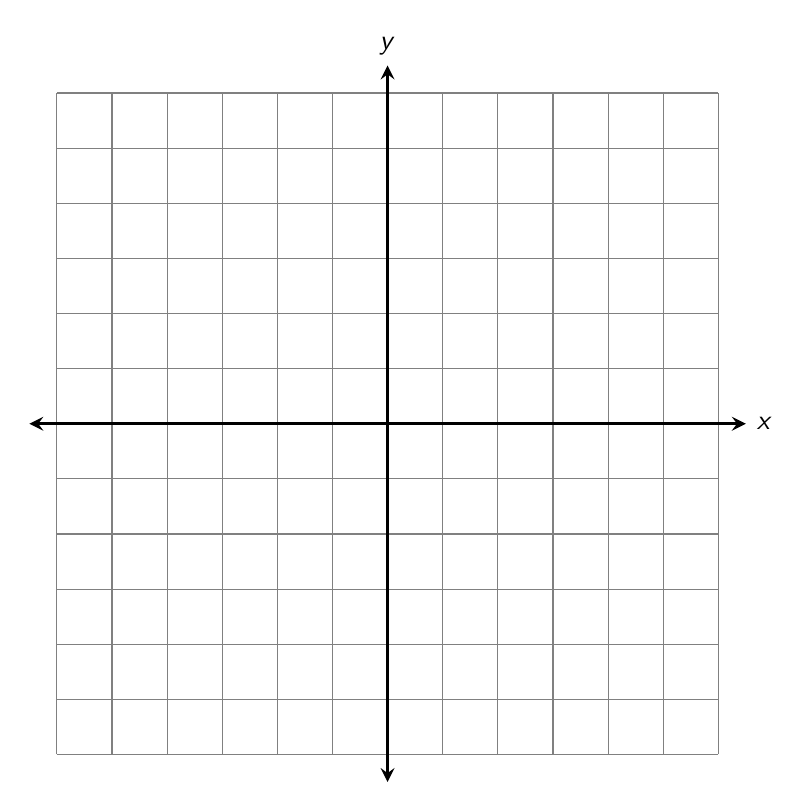
\begin{tikzpicture}[scale=0.7]
\draw[gray] (-6,-6) grid (6,6);
\draw[<->, very thick] (-6.5,0) -- (6.5,0) node [right] {$x$};
\draw[<->, very thick] (0,-6.5) -- (0,6.5) node [above] {$y$};
\end{tikzpicture}

\newpage


If we multiply our vector by $-1$, that will point the vector in the opposite direction.  \vspace{0.5in}

If $\vec{a} = \begin{bmatrix}
3 \\ -2
\end{bmatrix}$, what is $-1\vec{a}\,$? \bigskip

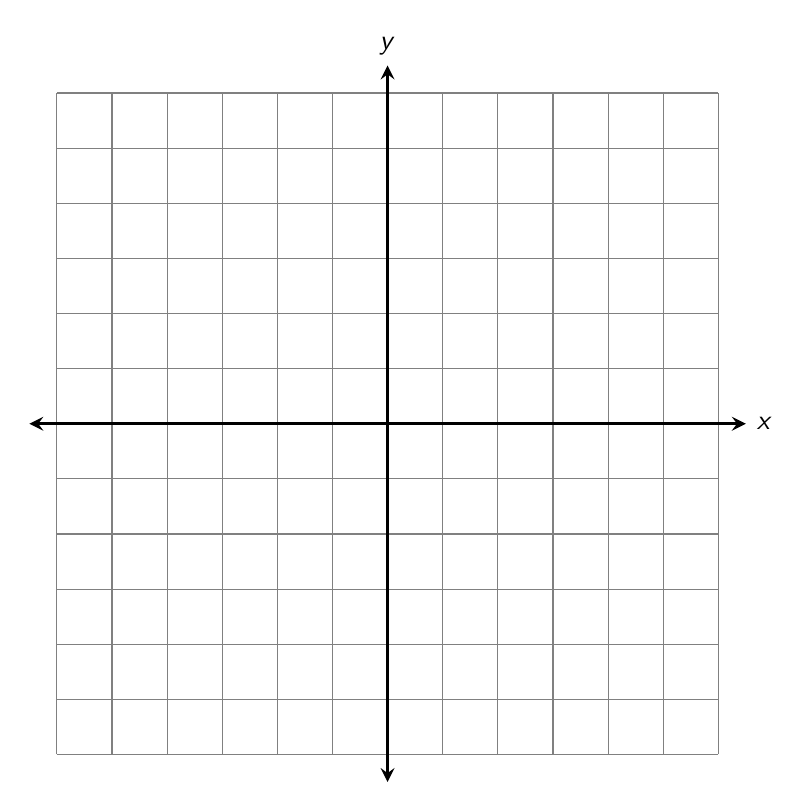
\begin{tikzpicture}[scale=0.7]
\draw[gray] (-6,-6) grid (6,6);
\draw[<->, very thick] (-6.5,0) -- (6.5,0) node [right] {$x$};
\draw[<->, very thick] (0,-6.5) -- (0,6.5) node [above] {$y$};
\end{tikzpicture}

\newpage

We can combine the scalar multiples with vector addition.   \vspace{0.5in}

{\color{red}\textbf{Example 2.}} Given $\vec{v} = \begin{bmatrix}
1 \\ -1 
\end{bmatrix}$ and $\vec{w} = \begin{bmatrix}
-2 \\ 0
\end{bmatrix}$ find and graph each. \vspace{0.25in}

(a) \quad $\vec{v} - \vec{w}$   \bigskip

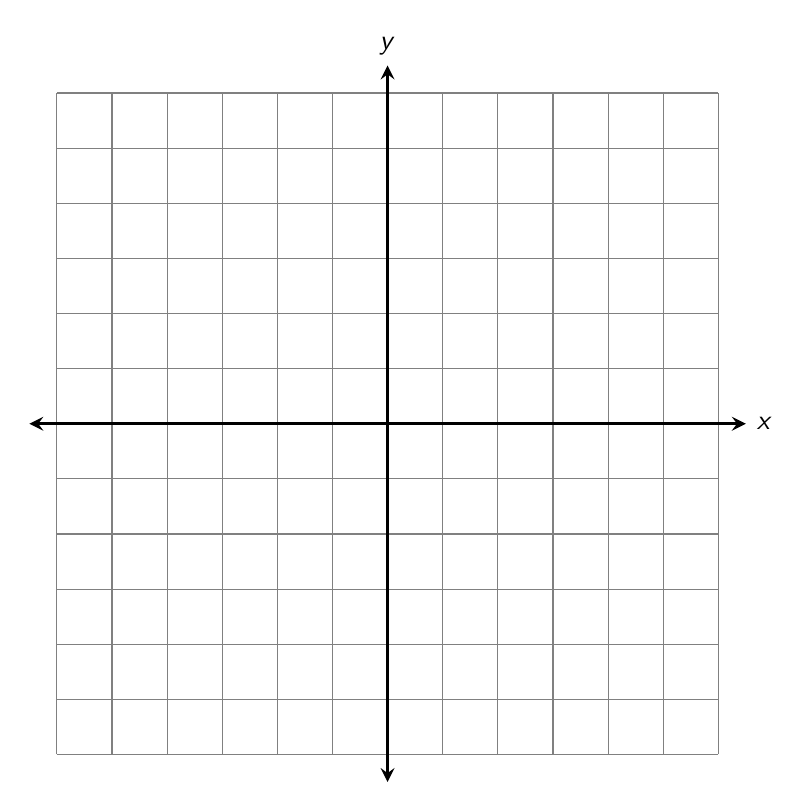
\begin{tikzpicture}[scale=0.7]
\draw[gray] (-6,-6) grid (6,6);
\draw[<->, very thick] (-6.5,0) -- (6.5,0) node [right] {$x$};
\draw[<->, very thick] (0,-6.5) -- (0,6.5) node [above] {$y$};
\end{tikzpicture}


\newpage

$\vec{v} = \begin{bmatrix}
1 \\ -1 
\end{bmatrix}$ and $\vec{w} = \begin{bmatrix}
-2 \\ 0
\end{bmatrix}$
\vspace{0.25in}


(b) \quad $3\vec{v} + \vec{w}$  \bigskip

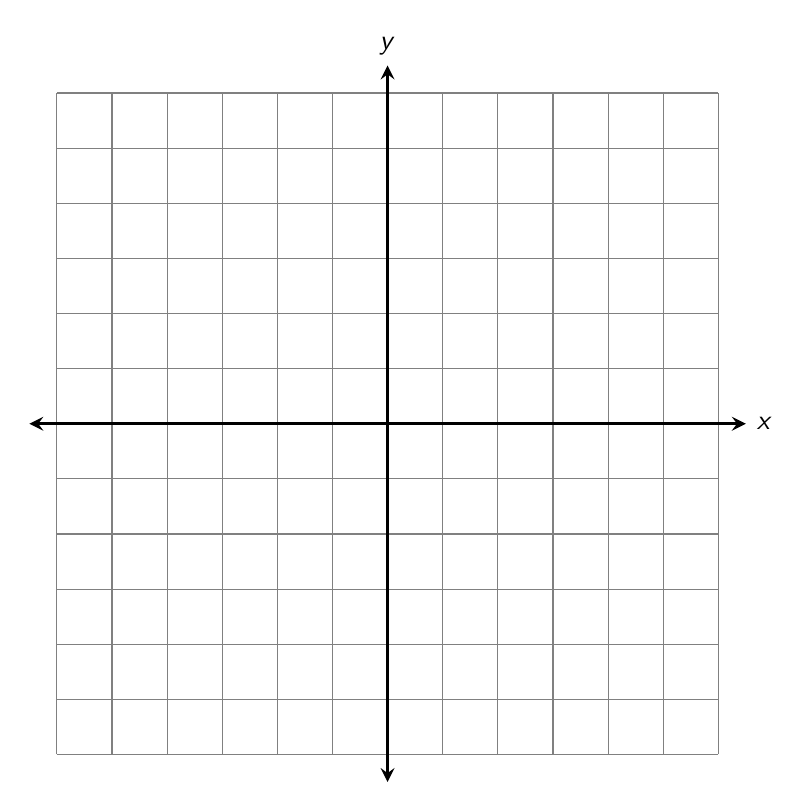
\begin{tikzpicture}[scale=0.7]
\draw[gray] (-6,-6) grid (6,6);
\draw[<->, very thick] (-6.5,0) -- (6.5,0) node [right] {$x$};
\draw[<->, very thick] (0,-6.5) -- (0,6.5) node [above] {$y$};
\end{tikzpicture}
\bigskip

(c) \quad $2\vec{v} - 1.5\vec{w}$   \bigskip

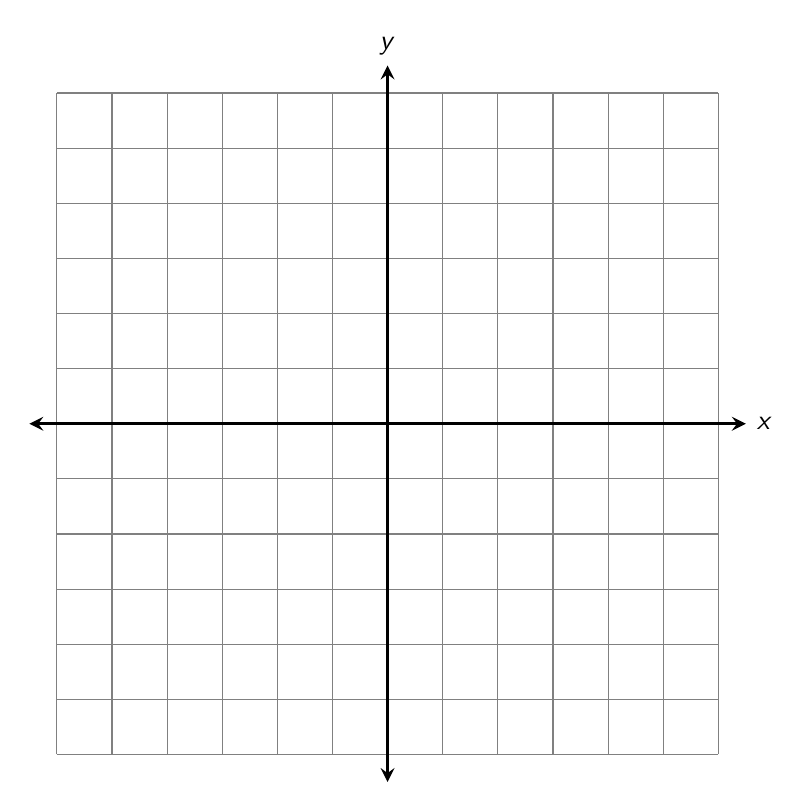
\begin{tikzpicture}[scale=0.7]
\draw[gray] (-6,-6) grid (6,6);
\draw[<->, very thick] (-6.5,0) -- (6.5,0) node [right] {$x$};
\draw[<->, very thick] (0,-6.5) -- (0,6.5) node [above] {$y$};
\end{tikzpicture}

\newpage

\subsubsection*{Basis Vectors $\hat{\imath}$ and $\hat{\jmath}$}
\bigskip

The basis vectors $\hat{\imath} = \begin{bmatrix} 1 \\ 0 \end{bmatrix}$ and $\hat{\jmath} = \begin{bmatrix} 0 \\ 1 \end{bmatrix}$ will serve as the foundation for matrix multiplication. \bigskip

\begin{tikzpicture}[scale=1.75]
\draw[gray] (-3,-3) grid (3,3);
\draw[<->, very thick] (-3.5,0) -- (3.5,0) node [right] {$x$};
\draw[<->, very thick] (0,-3.5) -- (0,3.5) node [above] {$y$};
\end{tikzpicture}

\newpage

Any vector can be written as a combination of a scalar and the basis vectors $\hat{\imath} \text{ and } \hat{\jmath}$. \vspace{1in}

For instance, $\vec{v} = \begin{bmatrix} 4 \\ 3 \end{bmatrix}$ can be written as follows:	\bigskip

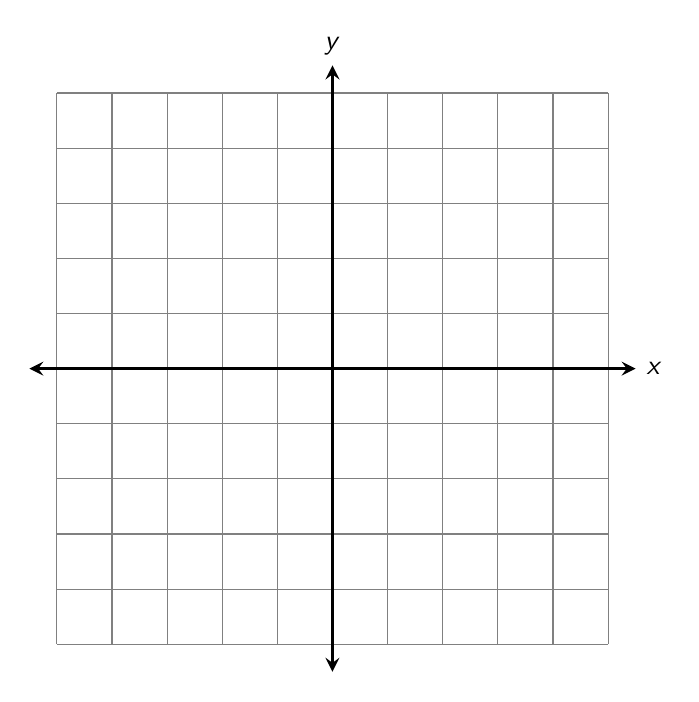
\begin{tikzpicture}[scale=0.7]
\draw[gray] (-5,-5) grid (5,5);
\draw[<->, very thick] (-5.5,0) -- (5.5,0) node [right] {$x$};
\draw[<->, very thick] (0,-5.5) -- (0,5.5) node [above] {$y$};
\end{tikzpicture}

\newpage


{\color{red}\textbf{Example 3.}} Write each in terms of basis vectors $\hat{\imath}$ and $\hat{\jmath}$.  \newline\\

(a) \quad $\vec{w} = \begin{bmatrix}
-3 \\ 1
\end{bmatrix}$
\vfill

(b) \quad $\vec{u} = \begin{bmatrix}
5 \\ -2
\end{bmatrix}$
\vfill

(c) \newline\\
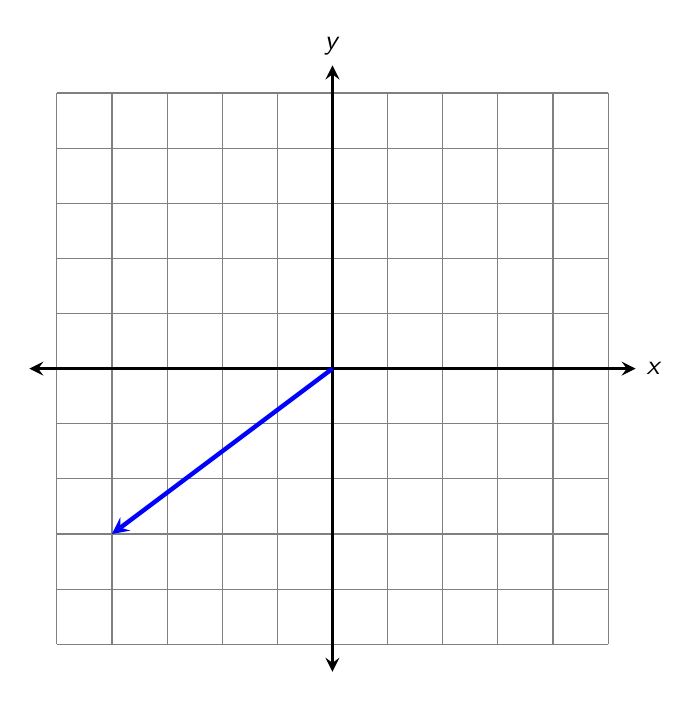
\begin{tikzpicture}[scale=0.7]
\draw[gray] (-5,-5) grid (5,5);
\draw[<->, very thick] (-5.5,0) -- (5.5,0) node [right] {$x$};
\draw[<->, very thick] (0,-5.5) -- (0,5.5) node [above] {$y$};
\draw[color=blue, ultra thick, ->] (0,0) -- (-4,-3);
\end{tikzpicture}
\vfill


\newpage

\subsection*{Matrices}

A \textbf{matrix} is a rectangular array of numbers. \newline\\
It can be composed of vectors (or possibly scalars).	\vspace{2in}

When listing the dimensions of a matrix, we note the number of rows, followed by the number of columns. 
\vspace{2in}

Matrix $A$ below has 3 rows and 4 columns, and has dimensions 3 by 4.
\[	A = \begin{bmatrix}
8 & 6 & 7 & 5 \\
3 & 0 & 9 & -2 \\
0 & 1 & -10 & 7 
\end{bmatrix}
\]
\vspace{1in}


Each of the values in a matrix are called \textbf{elements}. In matrix $A$, the element in the 1st row, 2nd column is 6 and is denoted
\[ a_{12} = 6 \]

\newpage

We can think of a matrix as several vectors in the coordinate plane. \vspace{0.5in}

\[
\begin{bmatrix}
{\color{blue}\bm{3}} & {\color{red}\bm{-1}} & {\color{violet}\bm{-5}} \\
{\color{blue}\bm{2}} & {\color{red}\bm{-4}} & {\color{violet}\bm{3}} 
\end{bmatrix}
\]
\begin{center}
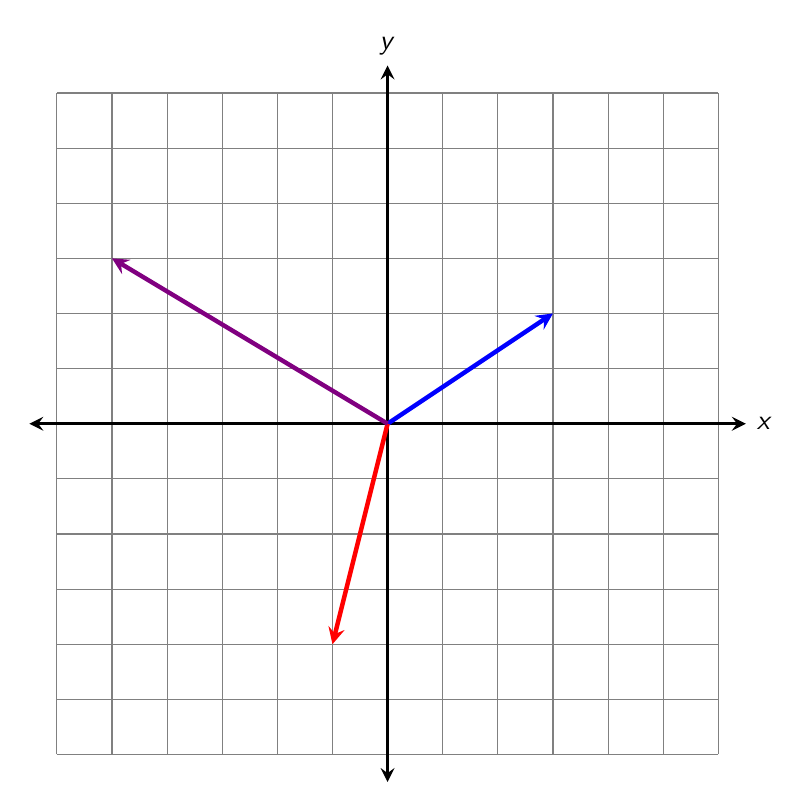
\begin{tikzpicture}[scale=0.7]
\draw[gray] (-6,-6) grid (6,6);
\draw[<->, very thick] (-6.5,0) -- (6.5,0) node [right] {$x$};
\draw[<->, very thick] (0,-6.5) -- (0,6.5) node [above] {$y$};
\draw[->, ultra thick, blue] (0,0) -- (3,2);
\draw[->, ultra thick, red] (0,0) -- (-1,-4);
\draw[->, ultra thick, violet] (0,0) -- (-5,3);
\end{tikzpicture}
\end{center}
\vfill

{\color{red}\textbf{Example 4.}} Graph the matrix $\begin{bmatrix}
1 & 0 \\
0 & 1
\end{bmatrix}$
\begin{center}
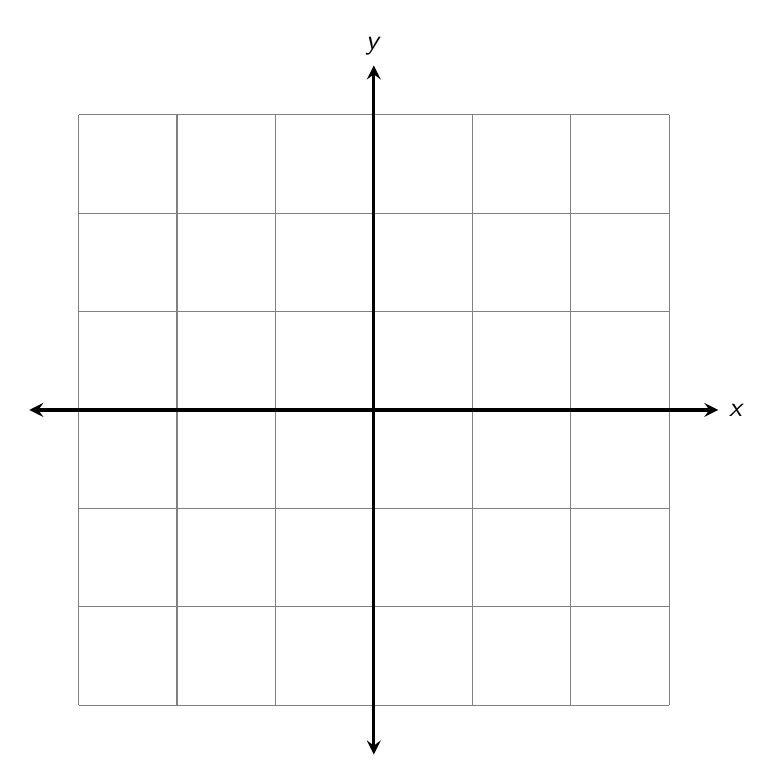
\begin{tikzpicture}[scale=1.25]
\draw[gray] (-3,-3) grid (3,3);
\draw[<->, very thick] (-3.5,0) -- (3.5,0) node [right] {$x$};
\draw[<->, very thick] (0,-3.5) -- (0,3.5) node [above] {$y$};
\end{tikzpicture}
\end{center}

\newpage

\subsubsection*{Matrix Addition and Subtraction}

If two matrices have the same dimensions, then we can add and subtract them. \newline\\

To do this, we add (or subtract) corresponding elements just like vector addition and subtraction.	\newline\\

{\color{red}\textbf{Example 5.}} Given matrices 
\[
A = \begin{bmatrix}
-2 & 3 \\
0 & 4 
\end{bmatrix}
\quad
B = \begin{bmatrix}
4 & -3 \\
-2 & -1
\end{bmatrix}
\quad
C = \begin{bmatrix}
-7 & 6 & -1 \\
0 & 4 & -4 
\end{bmatrix}
\]
find each and graph your answers (if possible).  \newline\\

(a) \quad $A + B$   \newline\\

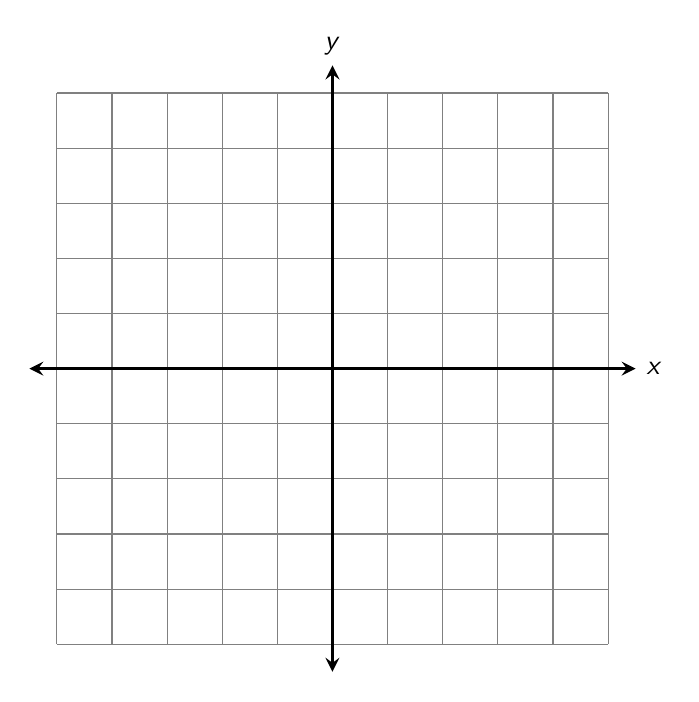
\begin{tikzpicture}[scale=0.7]
\draw[gray] (-5,-5) grid (5,5);
\draw[<->, very thick] (-5.5,0) -- (5.5,0) node [right] {$x$};
\draw[<->, very thick] (0,-5.5) -- (0,5.5) node [above] {$y$};
\end{tikzpicture}
\vfill

(b) \quad $B + A$   \newline\\
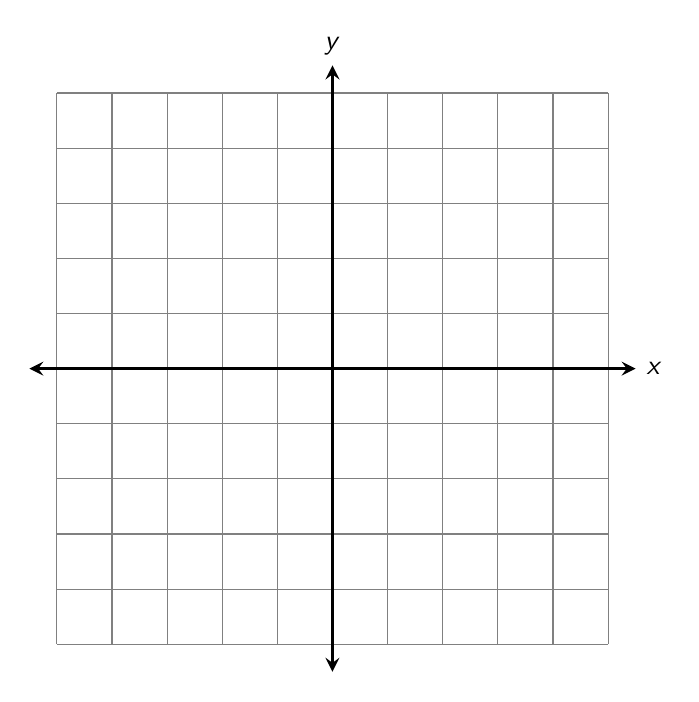
\begin{tikzpicture}[scale=0.7]
\draw[gray] (-5,-5) grid (5,5);
\draw[<->, very thick] (-5.5,0) -- (5.5,0) node [right] {$x$};
\draw[<->, very thick] (0,-5.5) -- (0,5.5) node [above] {$y$};
\end{tikzpicture}

\newpage

\[
A = \begin{bmatrix}
-2 & 3 \\
0 & 4 
\end{bmatrix}
\quad
B = \begin{bmatrix}
4 & -3 \\
-2 & -1
\end{bmatrix}
\quad
C = \begin{bmatrix}
-7 & 6 & -1 \\
0 & 4 & -4 
\end{bmatrix}
\]

(c) \quad $A - B$ \newline\\
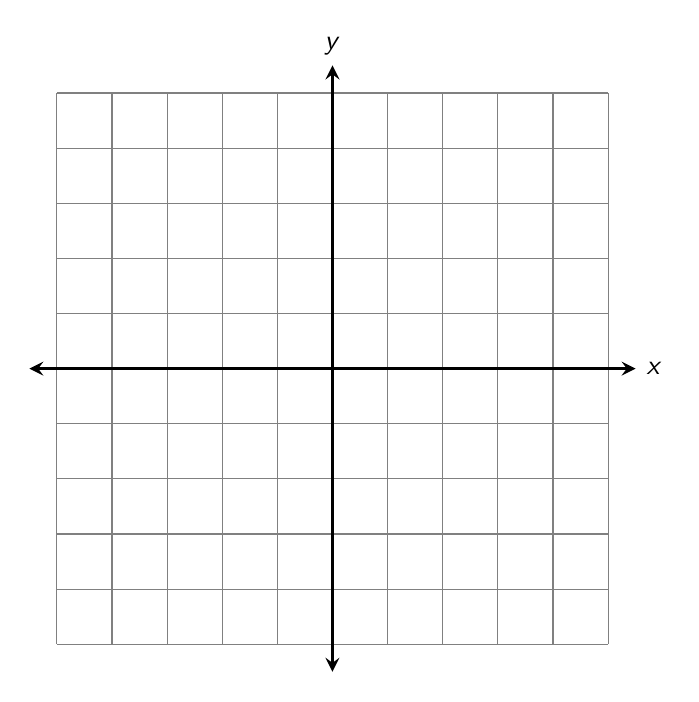
\begin{tikzpicture}[scale=0.7]
\draw[gray] (-5,-5) grid (5,5);
\draw[<->, very thick] (-5.5,0) -- (5.5,0) node [right] {$x$};
\draw[<->, very thick] (0,-5.5) -- (0,5.5) node [above] {$y$};
\end{tikzpicture}
\vfill

(d) \quad $A + C$ \newline\\
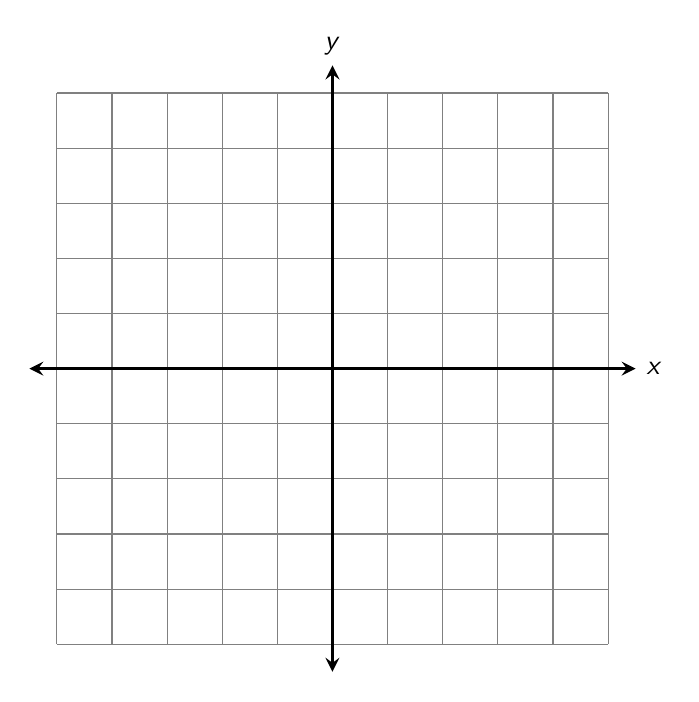
\begin{tikzpicture}[scale=0.7]
\draw[gray] (-5,-5) grid (5,5);
\draw[<->, very thick] (-5.5,0) -- (5.5,0) node [right] {$x$};
\draw[<->, very thick] (0,-5.5) -- (0,5.5) node [above] {$y$};
\end{tikzpicture}
\vfill 

\newpage

\subsubsection*{Scalar Multiplication}

We saw how scalars affect vectors. \newline\\

Since a matrix can be thought of as an array of vectors,

multiplying a matrix by a scalar has the same effect that multiplying a vector by a scalar does:  

\begin{center}
Each element in the matrix gets multiplied by the scalar.\end{center}

{\color{red}\textbf{Example 6.}} Using \[
A = \begin{bmatrix}
-2 & 3 \\
0 & 5 
\end{bmatrix}
\quad
B = \begin{bmatrix}
4 & -3 \\
-2 & -1
\end{bmatrix}
\quad
C = \begin{bmatrix}
-7 & 6 & -1 \\
0 & 4 & -4 
\end{bmatrix}
\]
find each.  \newline\\

(a) \quad $5A$  \vfill 
(b) \quad $-1C$ \vfill 
(c) \quad $5A + 2B$ \vfill 
 
\end{document}
